\chapter{Charged Particle Tracking}
\label{c:charged.track}

\bmad can track both charged particles and X-rays. This chapter deals
with charged particles and X-rays are handled in
chapter~\sref{c:xray.track}.

For tracking and transfer map calculations (here generically called
``tracking''), \bmad has various methods that can be applied to a
given element (Cf. Chapter~\sref{c:methods}). This chapter discusses
the \vn{bmad_standard} calculation that is the default for almost all
element types and the \vn{symp_lie_bmad} calculation that does
symplectic integration.

Generally, it will be assumed that tracking is in the forward direction.

%-------------------------------------------------------------------------
%-------------------------------------------------------------------------
\section{Element Coordinate System}
\label{s:ele.coords}

\index{element coordinates}
The general procedure for tracking through an element makes use of
\vn{element reference} coordinates (also called just \vn{element}
coordinates). Without any offsets, pitches or tilt, (henceforth
called ``misalignments''), the \vn{element} coordinates are the same
as the \vn{laboratory reference} coordinates (or simply \vn{laboratory}
coordinates) (\sref{s:ref}). The \vn{element} coordinates stay fixed
relative to the element. Therefore, if the element is misaliged, the
\vn{element coordinates} will follow as the element shifts in the
laboratory frame as shown in \fig{ele.coord}.

Tracking a particle through an element is a three step process:
\begin{enumerate}
\item
At the entrance end of the element, transform from the \vn{laboratory}
coordinates to the (entrance) \vn{element} coordinates.
\item
Track through the element ignoring any misalignments. 
\item
At the exit end of the element, transform from the (exit) \vn{element}
reference frame to the \vn{laboratory} reference frame.
\end{enumerate}

The transformation between \vn{laboratory} and \vn{element} reference
frames will depend upon whether the element is straight or not. In
any case, it is assumed that pitches are small so that second order
terms can be ignored.

%-------------------------------------------------------------------------

\begin{figure}[tb]
  \centering
  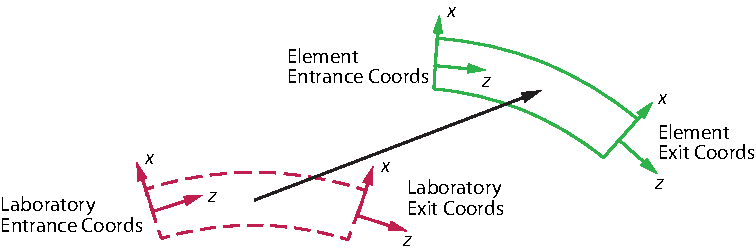
\includegraphics[width=5in]{coord-offset.pdf}
  \caption[Element Coordinate System.]
  {
\vn{Element} coordinates are coordinates attached to the pysical
element (solid green outline).  The \vn{laboratory} coordinates are
fixed at the nominal position of the element (red dashed outline).
  }
  \label{f:ele.coord}.
\end{figure}

%-------------------------------------------------------------------------
\subsection{Transform from Laboratory Entrace to Element Coordinates for Straight Elements}

The transformation from the laboratory coordinates to element
coordinates for an element that has a straight reference trajectory
through it is a two step process.
\begin{enumerate}
\setlength{\itemsep}{0pt}
\item
Track as in a drift a distance \vn{z_offset_tot}.
\item
Apply offsets and pitches
\vspace{-1ex}
\begin{align}
  x_1    &= x_0 - x_{\mbox{off}} + \frac{L}{2} \, x'_{pitch} \CRNO
  p_{x1} &= p_{x0} - (1 + p_{z0}) \, x'_{pitch} \CRNO
  y_1    &= y_0 - y_{\mbox{off}} + \frac{L}{2} \, y'_{pitch} \\
  p_{y1} &= p_{x0} - (1 + p_{z0}) \, y'_{pitch} \CRNO
  z_1    &= z_0 + x'_{pitch} \, x_1 + y'_{pitch} \, y_1 - 
    \frac{L}{4} (x^{\prime2}_{pitch} + y^{\prime2}_{pitch}) \nonumber
\end{align}
where $x'_{pitch}$ and $y'_{pitch}$ are the \vn{x_pitch_tot} and
\vn{y_pitch_tot} attributes of the element (\sref{s:offset}), and
$x_{\mbox{off}}$, and $y_{\mbox{off}}$ are the \vn{x_offset_tot} and
\vn{y_offset_tot} attributes.
Notice that $z_1$ is written in terms of $x_1$ and $y_1$
\item
Apply the tilt $\theta_t$ (\vn{tilt_tot})
\vspace{-1ex}
\begin{align}
  x_2    &=  x_1    \, \cos\theta_t + y_1    \, \sin\theta_t \CRNO
  p_{x2} &=  p_{x1} \, \cos\theta_t + p_{y1} \, \sin\theta_t \CRNO
  y_2    &= -x_1    \, \sin\theta_t + y_1    \, \cos\theta_t \\
  p_{y2} &= -p_{x1} \, \sin\theta_t + p_{y1} \, \cos\theta_t \nonumber
\end{align}
\end{enumerate}

%-------------------------------------------------------------------------
\subsection{Transform from Laboratory Entrace to Element Coordinates for Bend Elements}

Let $\bfr_c$ be the displacement of the bend at the bend center (where
offsets are specified (\sref{s:offset}).

The rotation matrix $\bfS_c$ transforming
from the center of the bend (where the misalignments are defined) to the
entrance face of the bend is
\begin{align}
  \bfS_c &= \bfW_\Psi^{-1} (\theta_t) \, \bfW_\Theta (\alpha_b/2) \, \bfW_\Psi (\theta_t) \\
\end{align}
where $\bfW_\Psi$ and $\bfW_\Theta$ are given by \Eqs{wtt0t},
$\theta_t$ is the \vn{ref_tilt} attribute of the bend and $\alpha_b$
is the bend \vn{angle}.

In the laboratory entrance coordinates, the pitches and offset are
\begin{align}
  \bfW &= \bfS \, 
    \begin{pmatrix}
      -y'_{pitch} \\ x'_{pitch} \\ 0
    \end{pmatrix} \\
  \bfV &= \bfS \, 
    \begin{pmatrix}
      x_{\mbox{off}} \\ y_{\mbox{off}} \\ z_{\mbox{off}} + 
    \end{pmatrix} +
    \bfS \, \bfL_c - \bfL_c
\end{align}
where the offset vector $\bfL_c$ is
\Begineq
  \bfL_c = \bfW_\Psi(\theta_t) \,
      \begin{pmatrix}
        2 \, \rho \, \sin^2 (\alpha_b / 2) \\ 0 \\ -\rho \, \sin(\alpha_b / 2)
      \end{pmatrix}
\Endeq

The transformation to element coordinates is then
\begin{enumerate}
\setlength{\itemsep}{0pt}
\item
\begin{align}
  x_1    &= x_0 - \bfV(1) \CRNO
  p_{x1} &= p_{x0} - \bfW(1) \, (1 + p_{z0}) \CRNO
  y_1    &= y_0 - \bfV(2) \\
  p_{y1} &= p_{x0} + \bfW(2) \, (1 + p_{z0}) \CRNO
  z_1    &= z_0 + \bfW(2) \, x_0 - \bfW(1) \, y_0 \nonumber
\end{align}
\item
Track as in a drift a distance $\bfV(3)$.
\item
Apply the non-reference shifting tilt $\theta_t$ (\vn{tilt_tot})
\vspace{-1ex}
\begin{align}
  x_2    &=  x_1    \, \cos\theta_t + y_1    \, \sin\theta_t \CRNO
  p_{x2} &=  p_{x1} \, \cos\theta_t + p_{y1} \, \sin\theta_t \CRNO
  y_2    &= -x_1    \, \sin\theta_t + y_1    \, \cos\theta_t \\
  p_{y2} &= -p_{x1} \, \sin\theta_t + p_{y1} \, \cos\theta_t \nonumber
\end{align}
\end{enumberate}

%-------------------------------------------------------------------------
\subsection{Transform from Element Exit to Laboratory Coordinate for Straight Elements}

The back transformation from element to laboratory coordinates is
accomplished by the transformation
\begin{enumerate}
\setlength{\itemsep}{0pt}
\item
Apply tilt $\theta_t$
\vspace{-1ex}
\begin{align}
  x_1    &=  x_0    \, \cos\theta_t - y_0    \, \sin\theta_t \CRNO
  p_{x1} &=  p_{x0} \, \cos\theta_t - p_{y0} \, \sin\theta_t \CRNO
  y_1    &=  x_0    \, \sin\theta_t + y_0    \, \cos\theta_t \\
  p_{y1} &=  p_{x0} \, \sin\theta_t + p_{y0} \, \cos\theta_t \nonumber
\end{align}
\item
Apply offsets and pitches
\vspace{-1ex}
\begin{align}
  x_2    &= x_1 + x_{\mbox{off}} + \frac{L}{2} x'_{pitch}     \CRNO
  p_{x2} &= p_{x1} + (1 + p_{z1}) \, x'_{pitch}        \CRNO
  y_2    &= y_1 + y_{\mbox{off}} + \frac{L}{2} y'_{pitch}     \\
  p_{y2} &= p_{x1} + (1 + p_{z1}) \, y'_{pitch}        \CRNO
  z_2    &= z_1 + x'_{pitch} \, x_1 + y'_{pitch} \, y_1 - 
    \frac{L}{4} (x^{\prime2}_{pitch} + y^{\prime2}_{pitch})      \nonumber
\end{align}
\item
Track as in a drift a distance \vn{-z_offset_tot}.
\end{enumerate}

%-------------------------------------------------------------------------
\subsection{Transform from Element Exit to Laboratory Coordinate for Bend Elements}

The back transformation from element to laboratory coordinates is
accomplished by the transformation
\begin{enumerate}
\setlength{\itemsep}{0pt}
\item
Apply non-reference shifting tilt $\theta_t$
\vspace{-1ex}
\begin{align}
  x_1    &=  x_0    \, \cos\theta_t - y_0    \, \sin\theta_t \CRNO
  p_{x1} &=  p_{x0} \, \cos\theta_t - p_{y0} \, \sin\theta_t \CRNO
  y_1    &=  x_0    \, \sin\theta_t + y_0    \, \cos\theta_t \\
  p_{y1} &=  p_{x0} \, \sin\theta_t + p_{y0} \, \cos\theta_t \nonumber
\end{align}
\item
Apply offsets and pitches
\vspace{-1ex}
\begin{align}
  x_1    &= x_0 + \bfV(1) \CRNO
  p_{x1} &= p_{x0} + \bfW(1) \, (1 + p_{z0}) \CRNO
  y_1    &= y_0 + \bfV(2) \\
  p_{y1} &= p_{x0} - \bfW(2) \, (1 + p_{z0}) \CRNO
  z_1    &= z_0 - \bfW(2) \, x_0 + \bfW(1) \, y_0 \nonumber
\end{align}
\item
Track as in a drift a distance \vn{-z_offset_tot}.
\end{enumerate}

%-------------------------------------------------------------------------
\section{Hamiltonian}
\label{s:mag.hamiltonian}
The time dependent Hamiltonian $H_t$ in the curvilinear coordinate system shown
in \fig{f:local.coords} is
\Begineq
  H_t = \wt\psi + \left[ \left( \frac{p_s - a_s}{1 + g\, x} \right)^2 + \wt m^2 + 
  (p_x - a_x)^2 + (p_y - a_y)^2 +  \right]^{1/2}
\Endeq
where $(p_x, p_y, p_s/(1+gx))$ are the momentum normalized by $P_0$,
$\rho$ being the local radius of curvature of the reference particle,
and $\wt m$, $\Bf a$ and $\wt\psi$ are the normalized mass, vector, and scalar
potentials:
\Begineq
  \wt m = \frac{m \, c^2}{c \, P_0} \qquad
  \left( a_x, a_y, \frac{a_s}{1+g \, x} \right) = \frac{q \, \Bf A}{P_0 \, c} \qquad 
  \wt\psi(x,y,z) = \frac{q \, \psi}{P_0 \, c}
\Endeq

The $s$-dependent Hamiltonian is obtained from $H_t$ by solving for
$-p_s$. For particles propagating in the positive $s$ direction the
$s$-dependent Hamiltonian is
\Begineq
  H_{s,E} = -(1 + g \, x) \sqrt{\wt E^2 - \wt m^2 - (p_x - a_x)^2 - (p_y - a_y)^2} - a_s
  \label{hse1gx1}
\Endeq
where $\wt E = E/c\, P_0$ is the normalized energy and the equation 
has been simplified by assuming that $\wt\psi$ is zero. Using a contact
transformation to convert to \bmad coordinates (\sref{s:phase.space}) gives
\Begineq
  H \equiv H_s = -(1 + g \, x) \sqrt{(1 + p_z)^2 - (p_x - a_x)^2 - (p_y - a_y)^2} - a_s +
  \frac{1}{\beta_0} \, \sqrt{(1+p_z)^2 + \wt m^2}
  \label{h1gx1}
\Endeq
where $\beta_0$ is the reference velocity. The last term on the RHS of
\Eq{h1gx1} accounts for the fact that the \bmad canonical $z$ (\Eq{zbctt})
has an ``extra'' term $\beta \, c \, t_0$ so that \bmad canonical $z$ is with
respect to the reference particle's $z$.

The equations
of motion are
\begin{equation}
  \frac{dq_i}{ds} = \frac{\partial H}{\partial p_i} \qquad
  \frac{dp_i}{ds} = -\frac{\partial H}{\partial q_i}
  \label{rshp}
\end{equation}

For backwards propagation, where $p_s$ is negative, solving for $p_s$ involves using
a different part of the squareroot branch. the Hamiltonian $H_{-s}$ is then
\Begineq
  H_{-s} = (1 + g \, x) \sqrt{(1 + p_z)^2 - (p_x - a_x)^2 - (p_y - a_y)^2} - a_s - 
  \frac{1}{\beta_0} \, \sqrt{(1+p_z)^2 + \wt m^2}
\Endeq

\label{paraxial approximation} 
Without an electric field, $\psi$ is zero. Assuming a non-curved
coordinate system ($g = 0$), and using the paraxial approximation
(\sref{s:phase.space}), \Eq{h1gx1} becomes
\Begineq
  H = \frac{(p_x - a_x)^2}{2 (1 + p_z)} + \frac{(p_y - a_y)^2}{2 (1 + p_z)} - 
  (1 + g \, x) \, a_s +   \frac{1}{\beta_0} \, \sqrt{(1+p_z)^2 + \wt m^2}
  \label{hpapa}
\Endeq

Once the transverse trajectory has been calculated, the longitudinal position
$z_2$ at the exit end of an element is obtained from symplectic
integration of \Eq{hpapa}
\Begineq
  z_2 = z_1 - \frac{1}{2 (1 + p_{z1})^2} \int \! ds \, 
  \left[ (p_x - a_x)^2 + (p_y - a_y)^2 \right] - \int \! ds \, g \, x
  \label{zz121p}
\Endeq
where $z_1$ is the longitudinal position at the entrance end of the element.
Using the equations of motion \Eqs{rshp} this can also be rewritten as
\Begineq
  z_2 = z_1 - \frac{1}{2} \int \! ds \, 
  \left[ \left( \frac{dx}{ds} \right)^2 + \left( \frac{dy}{ds} \right)^2 \right] - 
  \int \! ds \, g \, x
  \label{zz12sx}
\Endeq

For some elements, \vn{bmad_standard} uses a truncated Taylor map for
tracking.  For elements without electric fields where the particle
energy is a constant, the transfer map for a given coordinate $r_i$
may be expanded in a Taylor series
\Begineq
  r_{i,2} \rightarrow m_i + \sum_{j = 1}^4 m_{ij} \, r_{j,1} + 
  \sum_{j = 1}^4 \sum_{k = j}^4 m_{ijk} \, r_{j,1} \, r_{k,1} + \ldots
\Endeq
where the map coefficients $m_{ij\cdots}$ are functions of $p_z$.  For
linear elements, the transfer map is linear for the transverse
coordinates and quadratic for $r_i = z$.

Assuming mid--plane symmetry of the magnetic field, so
that $a_x$ and $a_y$ can be set to zero\cite{b:madphysics}, The vector
potential up to second order is (cf.~\Eq{byx0b})
\Begineq
  a_s = -k_0 \left( x - \frac{g \, x^2}{2 (1 + g\, x)} \right) -
  \frac{1}{2} k_1 \left( x^2 - y^2 \right)
  \label{akxgx}
\Endeq

%---------------------------------------------------------------------------------
%---------------------------------------------------------------------------------
\section{Symplectic Integration}
\label{s:symp.track}
\index{symplectic integration}

Using \Eq{hpapa} the Hamiltonian is written in the form
\Begineq
  H = H_x + H_y + H_z
\Endeq
where
\begin{equation}
  H_x = \frac{(p_x - a_x)^2}{2 (1 + \delta)}, \qquad
  H_y = \frac{(p_y - a_y)^2}{2 (1 + \delta)}, \qquad
  H_s = - a_s 
\end{equation}

For tracking, the element is broken up into a number of slices set by
the element's \vn{ds_step} attribute. For each slice, the tracking
uses a quadratic symplectic integrator $I$:
\Begineq
  I = T_{s/2} \; I_{x/2} \; I_{y/2} \; I_s \; I_{y/2} \; I_{x/2} \; T_{s/2}
\Endeq
$T_{s/2}$ is just a translation of the $s$ variable:
\Begineq
  s \rightarrow s + \frac{ds}{2}
\Endeq
And the other integrator components are
\begin{align}
  I_{x/2} &= \exp \left( : -\frac{ds}{2} H_x : \right) \CRNO
  I_{y/2} &= \exp \left( : -\frac{ds}{2} H_y : \right) \\
  I_{s}   &= \exp \left( : -ds \, H_s : \right) \nonumber
\end{align}
The evaluation of $I_{x/2}$ and $I_{y/2}$ is tricky since it involves both transverse
position and momentum variables. The trick is to split the integration into three parts.
For $I_{x/2}$ this is
\begin{align}
  I_{x/2} &= \exp \left( : -\frac{ds}{2} \frac{(p_x - A_x)^2}{2 (1 + \delta)} : \right) \CRNO
  &= \exp \left( : -\int A_x \, dx : \right) \,
     \exp \left( : -\frac{ds}{2} \frac{p_x^2}{2 (1 + \delta)} : \right) \,
     \exp \left( : \int A_x \, dx : \right)
  \label{ids2}
\end{align}
With an analogous expression for $I_{y/2}$.

\index{quadrupole}\index{sextupole}\index{wiggler}
For magnetic elements that do not have longitudinal fields
(quadrupoles, sextupoles, etc.), $a_x$ and $a_y$ can be taken to be
zero (cf.~\Eq{akxgx}). For wigglers (\sref{s:wiggler}), \bmad computes $\Bf A$ using
\begin{align}
  A_x(x,y,s) &= 0 \CRNO
  A_y(x,y,s) &=  \int_0^x d\wt x \, B_z(\wt x, y, s) 
  \label{a0a0a0} \\
  A_s(x,y,s) &= -\int_0^y d\wt x \, B_y(\wt x, y, s) \nonumber
\end{align}
given the form of the of the magnetic field of \Eqs{f1}, \eq{f2}, and
\eq{f3}, the integrals in \Eq{a0a0a0} and \eq{ids2} are easily calculated.

\index{lcavity}\index{rfcavity}
For \vn{lcavity} and \vn{rfcavity} elements, the vector potential is computed from
\Eq{aiew}.

%---------------------------------------------------------------------------------
%---------------------------------------------------------------------------------
\section{BeamBeam Element Tracking}
\label{s:beambeam.std}
\index{beambeam}

A beam-beam element (\sref{s:bbi}) simulates the effect on a tracked
particle of an opposing beam of particles moving in the opposite
direction. The opposing beam, called the ``strong'' beam, is assumed
to be Gaussian in shape.

The strong beam is divided up into \vn{n_slice} equal charge (not
equal thickness) slices. Propagation through the strong beam involves
a kick at the charge center of each slice with drifts in between the
kicks. The kicks are calculated using the standard Bassetti--Erskine
complex error function formula\cite{b:talman}.  Even though the strong
beam can have a finite \vn{sig_z} the length of the element is always
considered to be zero. This is achieved by adding drifts at either end
of any tracking so that the longitudinal starting point and ending
point are identical. The longitudinal $s$--position of the
\vn{BeamBeam} element is at the center of the strong bunch. For
example, with \vn{n_slice} = 2 the calculation would proceed as
follows:
\begin{enumerate}
  \item  Start with the reference particle at the center of the strong bunch.
  \item  Propagate (drift) backwards to the center of the first slice.
  \item  Apply the beam--beam kick due to the first slice.
  \item  Propagate (drift) forwards to the center of the second slice.
  \item  Apply the beam--beam kick due to the second slice.
  \item  Propagate (drift) backwards to end up with the reference particle
     at the center of the strong bunch.
\end{enumerate}

%---------------------------------------------------------------------------------
%---------------------------------------------------------------------------------
\section{Bend Element: Fringe Tracking}
\label{s:.bend.fringe.std}
\index{sbend}

The transformation for the entrance face of an \vn{sbend} is
\begin{align}
  p_{x2} &= p_{x1} + k_x \, x_1 \CRNO
  p_{y2} &= p_{y1} + k_y \, y_1
\end{align}
where
\begin{align}
  k_x &= g_{tot} \, \tan(e_1) \CRNO
  k_y &= -g_{tot} \, \tan \left[ e_1 - 2 \, |g_{tot}| \, f_{int} \,  h_{gap} \, 
    \frac{1 + \sin(e1)^2}{\cos(e_1)} \right]
\end{align}
where $g_{tot}$ is the total bending strength (design +
error). Similar equations are used for tracking the exit edge of the
bend.

%---------------------------------------------------------------------------------
%---------------------------------------------------------------------------------
\section{Bend Element: Body Tracking}
\label{s:bend.body.std}
\index{sbend}

The Hamiltonian for the body of an \vn{sbend} is
\Begineq
  H = (k_0 - g) x - g \, x \, p_z + 
  \frac{1}{2}\left( (k_1 + g \, k_0) x^2 - k_1 \, y^2 \right) +
  \frac{p_x^2 + p_y^2}{2 (1 + p_z)} 
\Endeq

This is simply solved
\begin{align}
  x_2    &= c_x \, (x - x_c) + s_x \, \frac{p_{x1}}{1 + p_{z1}} + x_c \CRNO
  p_{x2} &= \tau_x \, \om_x^2 \, \, (1 + p_{z1}) \, s_x \, (x -x_c) + c_x \, p_{x1} \CRNO
  y_2    &= c_y \, y_1 + s_y \, \frac{p_{y1}}{1 + p_{z1}} \CRNO
  p_{y2} &= \tau_y \, \om_y^2 \, \, (1 + p_{z1}) \, s_y \, y_1 + c_y \, p_{y1} \\
  z_2    &= z_1 + m_5 + m_{51} (x - x_c) + m_{52} p_{x1} + m_{511} \, (x-x_c)^2 \, + \CRNO
         &\hspace*{20ex} m_{512} \, (x-x_c) \, p_{x1} + m_{522} \, p_{x1}^2 + 
                         m_{533} \, y^2 + m_{534} \, y_1 \, p_{y1} + m_{544} \, p_{y1}^2 \CRNO
  p_{z2} &= p_{z1} \nonumber
\end{align}
where 
\begin{alignat}{2}
  k_x &= k_1 + g \, k_0 & \qqquad
  \om_x &\equiv \sqrt{\frac{|k_x|}{1 + p_{z1}}} \CRNO
  x_c &= \frac{g \, (1 + p_{z1}) - k_0}{k_x} & \qqquad
  \om_y &\equiv \sqrt{\frac{|k_1|}{1 + p_{z1}}} 
\end{alignat}
and
\begin{alignat}{6}
         &\hspace*{3ex}  && k_x > 0          &\hspace*{3ex}& k_x < 0 & \qqquad
         &\hspace*{3ex}  && k_1 > 0          &\hspace*{3ex}& k_1 < 0 \CRNO
     c_x &=   && \cos  (\om_x \, L)               && \cosh (\om_x \, L) & \qqquad
     c_y &=   && \cosh (\om_y \, L)               && \cos  (\om_y \, L) \CRNO
     s_x &=   && \frac{\sin  (\om_x \, L)}{\om_x} && \frac{\sinh (\om_x \, L)}{\om_x} & \qqquad
     s_y &=   && \frac{\sinh (\om_y \, L)}{\om_y} && \frac{\sin  (\om_y \, L)}{\om_y} \\
  \tau_x &=   && {-}1             && {+}1             & \qqquad
  \tau_y &=   && {+}1             && {-}1             \nonumber
\end{alignat}
and
\begin{alignat}{2}
  m_5     &= -g \, x_c \, L & \qqquad & \CRNO
  m_{51}  &= -g \, s_x & \qqquad
  m_{52}  &= \frac{\tau_x \, g}{1 + p_{z1}} \, \frac{1 - c_x}{\om_x^2} \CRNO
  m_{511} &= \frac{\tau_x \,\, \om_x^2}{4} \, (L - c_x \, s_x) & \qqquad
  m_{533} &= \frac{\tau_y \,\, \om_y^2}{4} \, (L - c_y \, s_y) \CRNO
  m_{512} &= \frac{-\tau_x \,\, \om_x^2}{2 \, (1 + p_{z1})} \, s_x^2 & \qqquad
  m_{534} &= \frac{-\tau_y \,\, \om_y^2}{2 \, (1 + p_{z1})} \, s_y^2 \CRNO
  m_{522} &= \frac{-1}{4 \, (1 + p_{z1})^2} \, (L + c_x \, s_x) & \qqquad
  m_{544} &= \frac{-1}{4 \, (1 + p_{z1})^2} \, (L + c_y \, s_y) \nonumber
\end{alignat}

%---------------------------------------------------------------------------------
%---------------------------------------------------------------------------------
\section{Drift Element Tracking}
\label{s:drift.std}
\index{drift} 

\Eq{h1gx1} for a drift has $\Bf a = 0$ and $g = 0$. The Hamiltonian for a
drift is then
\Begineq
  H = \frac{p_x^2 + p_y^2}{2 (1 + p_z)} 
\Endeq
This gives the map
\begin{align}
  x_2    &= x_1 + \frac{L \, p_{x1}}{1 + p_{z1}} \CRNO
  p_{x2} &= p_{x1}  \CRNO
  y_2    &= y_1 + \frac{L \, p_{y1}}{1 + p_{z1}} \CRNO
  p_{y2} &= p_{y1}  \\
  z_2    &= z_1 - \frac{L \, (p_{x1}^2 + p_{y1}^2)}{2 (1 + p_{z1})^2} \CRNO
  p_{z2} &= p_{z1} \nonumber
\end{align}

%---------------------------------------------------------------------------------
%---------------------------------------------------------------------------------
\section{Kicker, Hkicker, Vkicker, and Elseparator Element Tracking}
\label{s:kicker.std}
\index{kicker}
\index{hkicker}
\index{vkicker}
\index{elseparator}

The Hamiltonian for a horizontally deflecting kicker or separator is
\Begineq
  H = \frac{p_x^2 + p_y^2}{2 (1 + p_z)} - k_0 \, x 
\Endeq
This gives the map
\begin{align}
  x_2    &= x_1 + \frac{1}{1 + p_{z1}} \, \left( L \, p_{x1} + \frac{1}{2} k_0 \, L^2 \right) \CRNO
  p_{x2} &= p_{x1} + k_0 \, L \CRNO
  y_2    &= y_1 + \frac{L \, p_{y1}}{1 + p_{z1}} \CRNO
  p_{y2} &= p_{y1}  \\
  z_2    &= z_1 - \frac{L}{2 (1 + p_{z1})^2} \, 
    \left( p_{x1}^2 + p_{y1}^2 + p_{x1} \, k_0 \, L + \frac{1}{3} k_0^2 \, L^2 \right) \CRNO
  p_{z2} &= p_{z1} \nonumber
\end{align}
The generalization when the kick is not in the horizontal plane is easily derived.

%---------------------------------------------------------------------------------
%---------------------------------------------------------------------------------
\section{Lcavity Element Tracking}
\label{s:lcavity.std}
\index{lcavity}

The transverse trajectory through an \vn{Lcavity} is modeled using equations
developed by Rosenzweig and Serafini\cite{b:rosenzweig} (R\&S) with
\begin{align}
  b_0 &= 1 \CRNO
  b_{-1} &= 1 
\end{align}
and all other $b_n$ set to zero.

The transport equations in R\&S were developed in the
ulta-relativistic limit with $\beta = 1$.  To extend these equations,
the transport through the cavity body (R\&S Eq.~(9)) has been modified
to give the correct phase-space area at non ultra-relativistic
energies:
\Begineq
  \begin{pmatrix}
    x \\ 
    x'
  \end{pmatrix}_2 = 
  \begin{pmatrix}
    \cos(\alpha)  &  
    \sqrt{\frac{8}{\eta(\Delta\phi)}} \, \frac{\beta_1 \, \gamma_1}{\gamma'} \, 
                                                   \cos(\Delta\phi) \, \sin(\alpha) \\
    -\sqrt{\frac{\eta(\Delta\phi)}{8}} \, 
                     \frac{\gamma'}{\beta_2 \, \gamma_2 \, \cos(\Delta\phi)} \, \sin(\alpha) &
    \frac{\beta_1 \, \gamma_1}{\beta_2 \, \gamma_2} \, \cos(\alpha)
  \end{pmatrix}
  \,
  \begin{pmatrix}
    x \\ 
    x'
  \end{pmatrix}_1
\Endeq
The added factors of $\beta$ give the matrix the correct determinate
of $\beta_1 \, \gamma_1 / \beta_2 \, \gamma_2$. {\em While the added
factors of $\beta$ do correct the phase space area, the above equation
can only be considered as a rough approximation for simulating
particles when $\beta$ is significantly different from 1. Indeed, the
only accurate way to simulate such particles is by integrating through
the actual field [Cf.~Runge Kutta tracking (\sref{s:tkm})]}

The change in $z$ going through a cavity is calculated by first calculating the particle
transit time $\Delta t$
\begin{align}
  c \, \Delta t &= \int_{s_1}^{s_2} \!\! ds \,\, \frac{1}{\beta(s)} \CRNO
  &= \int_{s_1}^{s_2} \!\! ds \, \frac{E}{\sqrt{E^2 - (mc^2)^2}} \\
  &= \frac{c \, P_{z2} - c \, P_{z1}}{G} \nonumber
\end{align}
where it has been assumed that the accelerating gradient $G$ is
constant through the cavity. In this equation $\beta = v / c$, $E$ is
the energy, and $P_{z1}$ and $P_{z2}$ are the entrance and exit
momenta. Using \Eq{zbctt}, the change in $z$ is thus
\Begineq
  z_2 = \frac{\beta_2}{\beta_1} \, z_1 - 
  \beta_2 \, 
  \left(
  \frac{c \, P_{z2} - c \, P_{z1}}{G} - 
  \frac{c \, \Pbar_{z2} - c \, \Pbar_{z1}}{\BAR G}
  \right)
\Endeq
where $\Pbar$ and $\BAR G$ are the momentum and gradient of the
reference particle.

Note that the above transport equations are only symplectic on-axis
There are second order terms in the transverse coordinates that are
missing. To obtain a proper symplectic matrix, the \vn{symplectify}
attirubte of an \vn{lcavity} element (\sref{s:symp}) can be set to
True.

%---------------------------------------------------------------------------------
%---------------------------------------------------------------------------------
\section{Mirror Element Tracking}
\label{s:mirror.std}
\index{mirror}

%---------------------------------------------------------------------------------
%---------------------------------------------------------------------------------
\section{Octupole Element Tracking}
\label{s:octupole.std}
\index{octupole}

The Hamiltonian for an upright octupole is
\Begineq
  H = \frac{p_x^2 + p_y^2}{2 (1 + p_z)} + \frac{k_3}{24} (x^4 - 6 \, x^2 \, y^2 + y^4)
\Endeq

An octupole is modeled using a kick-drift-kick model.

%---------------------------------------------------------------------------------
%---------------------------------------------------------------------------------
\section{Patch Element Tracking}
\label{s:patch.std}
\index{patch}

\begin{figure}[tb]
  \centering
  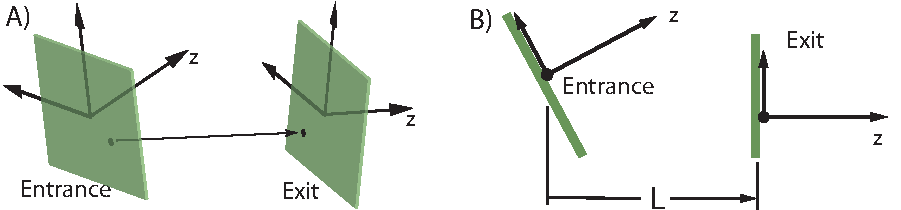
\includegraphics[width=5in]{patch.pdf}
  \caption[Standard patch transformation.]
{Standard tracking through a patch element. A particle's starting coordinate at
the entrance end of the patch has, by construction, coordinate $z$ =
0. The particle is drifted, as in a field free region, between the
entrance $z = 0$ plane and the exit $z = 0$ plane.}
  \label{f:patch.track}
\end{figure}

%---------------------------------------------------------------------------------

The transformation of the reference coordinates through a ``standard''
patch (a patch where custom fields are not used) is given by
\Eqs{vwlv} and \eq{wws}. At the entrance end of the patch, a
particle's position and momentum in the entrance coordinate system will be
\begin{alignat}{1}
  \bfr &= (x, y, 0) \CRNO
  \bfP &= (P_x, P_y, P_z) = 
    \left( p_x, p_y, \pm \sqrt{(1+p_z)^2 - p_x^2 - p_y^2} \right) \, P_{0\text{ent}}
\end{alignat}
where $p_x$, $p_y$ and $p_z$ are the phase space momenta, and $z$,
which is coordinate $z$ and not phase space $z$, is always zero by
construction as shown in \fig{f:patch.track} [Also see \fig{f:local.coords}
and the discussion in \sref{s:phase.space}.] The sign of the
longitudinal momentum $P_z$ is determined by whether the particle is
traveling in the positive $s$ or negative $s$ direction (which will
occur when an element is flipped longitudinally).

The transformation between entrance and exit coordinate systems is given by \Eqs{rwlr} and \eq{pps}
\begin{alignat}{1}
  \bfr &\rightarrow 
    \bfS^{-1} \, (\bfr - \bfL) \CRNO
  \bfP &\rightarrow \bfS^{-1} \, \bfP
\end{alignat}
where $\bf L$ is given by \Eq{lxyz}
\begin{example}
  \(\bf L\) =  (x_offset, y_offset, z_offset)
  \label{lxyz2}
\end{example}

After this transformation, the particle must be propagated by a longitudinal length
$-r_z$ to intersect the $r_z = 0$ plane of the exit face.
\begin{alignat}{1}
  \bfr &\rightarrow (r_x - r_z \, \frac{P_x}{P_z}, r_y - r_z \, \frac{P_y}{P_z}, 0) \CRNO
  \bfP &\rightarrow \bfP
\end{alignat}

The final $\bfr$ and $\bfP$ can now be used compute the particles
phase space coordinates, along with the time $t$ and the reference time
$t_{\text{ref}}$ at the exit end.
\begin{alignat}{3}
  x &\rightarrow r_x \qquad &p_x &\rightarrow \frac{P_x}{P_{0\text{exi}}} \CRNO
  y &\rightarrow r_y \qquad &p_y &\rightarrow \frac{P_y}{P_{0\text{exi}}} \\
  z &\rightarrow z + r_z \, \frac{|\bfP|}{P_z} + L_0 \, \frac{\beta}{\beta_0} +
    \beta \, \text{t_offset} \qquad
    &p_z &\rightarrow \frac{(1+p_z) \, P_{0\text{ent}} - P_{0\text{exi}}}{P_{0\text{exi}}} \CRNO
  t &\rightarrow t - r_z \, \frac{|\bfP|}{P_z \, \beta} \qquad
  &t_{\text{ref}} &\rightarrow t_{\text{ref}} + \text{t_offset} + L_0 \, \frac{1}{\beta_0} \nonumber
\end{alignat}
where the exit reference momentum $P_{0\text{exi}}$ is related to the
entrance reference momentum $P_{0\text{ent}}$ through
\vn{e_tot_offset}.  In the above equation, $\beta$ is the particle
velocity, $\beta_0$ is the velocity of the reference particle, and
$L_0$ is the drift length of the reference particle
\Begineq
  L_0 = \frac{1}{S^{-1}_{33}} \, \left( 
  S^{-1}_{31} \, \text{x_offset} + S^{-1}_{32} \, \text{y_offset} + S^{-1}_{33} \, \text{z_offset}
  \right)
\Endeq

%---------------------------------------------------------------------------------
%---------------------------------------------------------------------------------
\section{Quadrupole Element Tracking}
\label{s:quadrupole.std}
\index{quadrupole}

The \vn{bmad_standard} calculates the transfer map through an upright
quadrupole and then transforms that map to the laboratory frame.

The Hamiltonian for an upright quadrupole is
\Begineq
  H = \frac{p_x^2 + p_y^2}{2 (1 + p_z)} + \frac{k_1}{2} (x^2 - y^2)
\Endeq
This is simply solved
\begin{align}
  x_2    &= c_x \, x_1 + s_x \, \frac{p_{x1}}{1 + p_{z1}} \CRNO
  p_{x2} &= \tau_x \, \om^2 \, \, (1 + p_{z1}) \, s_x \, x_1 + c_x \, p_{x1} \CRNO
  y_2    &= c_y \, y_1 + s_y \, \frac{p_{y1}}{1 + p_{z1}} \CRNO
  p_{y2} &= \tau_y \, \om^2 \, \, (1 + p_{z1}) \, s_y \, y_1 + c_y \, p_{y1} \\
  z_2    &= z_1 + m_{511} \, x_1^2 + m_{512} \, x_1 \, p_{x1} + m_{522} \, p_{x1}^2 + 
                   m_{533} \, y_1^2 + m_{534} \, y_1 \, p_{y1} + m_{544} \, p_{y1}^2 \CRNO
  p_{z2} &= p_{z1} \nonumber
\end{align}
where 
\Begineq
  \om \equiv \sqrt{\frac{|k_1|}{1 + p_{z1}}}
\Endeq
and
\begin{alignat}{6}
         &\hspace*{3ex}  && k_1 > 0          &\hspace*{3ex}& k_1 < 0 & \qqquad
         &\hspace*{3ex}  && k_1 > 0          &\hspace*{3ex}& k_1 < 0 \CRNO
     c_x &=   && \cos  (\om \, L) && \cosh (\om \, L) & \qqquad
     c_y &=   && \cosh (\om \, L) && \cos  (\om \, L) \CRNO
     s_x &=   && \frac{\sin  (\om \, L)}{\om} && \frac{\sinh (\om \, L)}{\om} & \qqquad
     s_y &=   && \frac{\sinh (\om \, L)}{\om} && \frac{\sin  (\om \, L)}{\om} \\
  \tau_x &=   && {-}1             && {+}1             & \qqquad
  \tau_y &=   && {+}1             && {-}1             \nonumber
\end{alignat}
with this
\begin{alignat}{2}
  m_{511} &= \frac{\tau_x \,\, \om^2}{4} \, (L - c_x \, s_x) & \qqquad
  m_{533} &= \frac{\tau_y \,\, \om^2}{4} \, (L - c_y \, s_y) \CRNO
  m_{512} &= \frac{-\tau_x \,\, \om^2}{2 \, (1 + p_{z1})} \, s_x^2 & \qqquad
  m_{534} &= \frac{-\tau_y \,\, \om^2}{2 \, (1 + p_{z1})} \, s_y^2 \\
  m_{522} &= \frac{-1}{4 \, (1 + p_{z1})^2} \, (L + c_x \, s_x) & \qqquad
  m_{544} &= \frac{-1}{4 \, (1 + p_{z1})^2} \, (L + c_y \, s_y) \nonumber
\end{alignat}

%---------------------------------------------------------------------------------
%---------------------------------------------------------------------------------
\section{RFcavity Element Tracking}
\label{s:rfcavity.std}
\index{rfcavity}

Tracking through an rfcavity uses a kick-drift-kick model. The kick is
a pure energy kick (see equations in \sref{s:rfcav}) and the phase of
the RF is calculated under the assumption that the waveform moves at a
phase velocity equal to the velocity of the reference particle.

\index{lcavity}
The transverse forces due to the RF are ignored. This is a resonable
approximation when the acceleration is small. \vn{Lcavity} elements
should be used in place of \vn{rfcavity} elements when this is not so.

%---------------------------------------------------------------------------------
%---------------------------------------------------------------------------------
\section{Sextupole Element Tracking}
\label{s:sextupole.std}
\index{sextupole}

The Hamiltonian for an upright sextupole is
\Begineq
  H = \frac{p_x^2 + p_y^2}{2 (1 + p_z)} + \frac{k_2}{6} (x^3 - 3 \, x \, y^2)
\Endeq

Tracking through a sextupole uses a kick-drift-kick model.

%---------------------------------------------------------------------------------
%---------------------------------------------------------------------------------
\section{Sol\_Quad Element Tracking}
\label{s:sol.quad.std}
\index{sol_quad}

The Hamiltonian is
\Begineq
  H = \frac{(p_x + \frac{k_s }{2}\, y)^2}{2 (1 + p_z)} + 
  \frac{(p_y - \frac{k_s}{2} \, x)^2}{2 (1 + p_z)} + \frac{k_1}{2} (x^2 - y^2)
\Endeq
Solving the equations of motion gives
\begin{align}
  x_2    &= m_{11} \, x_1 + m_{12} \, p_{x1} + m_{13} \, y_1 + m_{14} \, p_{y1} \CRNO
  p_{x2} &= m_{21} \, x_1 + m_{22} \, p_{x1} + m_{23} \, y_1 + m_{24} \, p_{y1} \CRNO
  y_2    &= m_{31} \, x_1 + m_{32} \, p_{x1} + m_{33} \, y_1 + m_{34} \, p_{y1} \CRNO
  p_{y2} &= m_{41} \, x_1 + m_{42} \, p_{x1} + m_{43} \, y_1 + m_{44} \, p_{y1} \\
  z_2    &= z_1 + \sum_{j = 1}^4 \sum_{k = j}^4 m_{5jk} \, r_j \, r_k  \CRNO
  p_{z2} &= p_{z1} \nonumber
\end{align}
where
\begin{alignat}{2}
  m_{11} &= \frac{1}{2 \, f} \, \left( f_{0+} \, c + f_{0-} \, c_h \right) & \qqquad
  m_{31} &= -m_{24} \CRNO
  m_{12} &= \frac{1}{2 \, f \, (1 + p_{z1})} \, 
            \left( \frac{f_{++}}{\om_+} \,  s + \frac{f_{--}}{\om_-} \, s_h \right) & \qqquad
  m_{32} &= -m_{14} \CRNO
  m_{13} &= \frac{\ks}{4 \, f} \, 
            \left( \frac{f_{+-}}{\om_+} \, s +\frac{f_{-+}}{\om_-} \, s_h \right) & \qqquad
  m_{33} &= \frac{1}{2 \, f} \, \left( f_{0-} \, c + f_{0+} \, c_h \right) \CRNO
  m_{14} &= \frac{\ks}{f \, (1 + p_{z1})} \, \left( -c + c_h \right) & \qqquad
  m_{34} &= \frac{1}{2 \, f \, (1 + p_{z1})} \, 
            \left( \frac{f_{+-}}{\om_+} \, s + \frac{f_{-+}}{\om_-} \, s_h \right) \CRNO
  m_{21} &= \frac{-(1 + p_{z1})}{8 \, f} \, 
            \left( \frac{\xi_{1+}}{\om_+} \, s + \frac{\xi_{2+}}{\om_-} s_h \right) & \qqquad
  m_{41} &= -m_{23} \\
  m_{22} &= m_{11} & \qqquad
  m_{42} &= -m_{13} \CRNO
  m_{23} &= \frac{\ks^3 \, (1 + p_{z1})}{4 \, f} \, \left( c - c_h \right) & \qqquad
  m_{43} &= \frac{-(1 + p_{z1})}{8 \, f} \, 
            \left( \frac{\xi_{1-}}{\om_+} \, s + \frac{\xi_{2-}}{\om_-} \, s_h \right) \CRNO
  m_{24} &= \frac{\ks}{4 \, f} \, 
            \left( \frac{f_{++}}{\om_+} \, s + \frac{f_{--}}{\om_-} \, s_h \right) & \qqquad
  m_{44} &= m_{33} \nonumber
\end{alignat}
and
\begin{alignat}{2}
  \kone        &= \frac{k_1}{1 + p_{z1}} & \qqquad 
  \ks          &= \frac{k_s}{1 + p_{z1}} \CRNO
  f            &= \sqrt{\ks^4 + 4 \, \kone^2} & \qqquad
  f_{\pm0}     &= f \pm \ks^2 \CRNO
  f_{0\pm}     &= f \pm 2 \, \kone & \qqquad
  f_{\pm\pm}   &= f \pm \ks^2 \pm 2 \, \kone \CRNO
  \om_+        &= \sqrt{\frac{f_{+0}}{2}} & \qqquad
  \om_-        &= \sqrt{\frac{f_{-0}}{2}} \\
  s            &= \sin (\om_+ \, L) & \qqquad
  s_h          &= \sinh (\om_- \, L) \CRNO
  c            &= \cos (\om_+ \, L) & \qqquad
  c_h          &= \cosh (\om_- \, L) \CRNO
  \xi_{1\pm} &= \ks^2 \, f_{+\mp} \pm 4 \, \kone \, f_{+\pm} & \qqquad
  \xi_{2\pm} &= \ks^2 \, f_{-\pm} \pm 4 \, \kone \, f_{-\mp} \nonumber
\end{alignat}

The $m_{5jk}$ terms are obtained via \Eq{zz121p}
\begin{align}
  m_{5jk} = - \frac{\tau_{jk}}{2 (1 + p_{z1})^2} \int \! ds \, 
  & \left[ 
    \left( m_{2j} + \frac{k_s}{2} \, m_{3j} \right) \, 
    \left( m_{2k} + \frac{k_s}{2} \, m_{3k} \right)   
  \right. + \\
  & \hspace*{15ex} \left.
    \left( m_{4j} - \frac{k_s}{2} \, m_{1j} \right) \, 
    \left( m_{4k} - \frac{k_s}{2} \, m_{1k} \right) 
  \right] \nonumber
\end{align}
where
\Begineq
  \tau_{jk} = 
  \begin{cases}
    1 & j = k \\
    2 & j \ne k 
  \end{cases}
\Endeq
The needed integrals involve the product of two trigonometric or
hyperbolic functions. These integrals are trivial to do but the
explicit equations for $m_{5jk}$ are quite long and in the interests of
brevity are not reproduced here.

%---------------------------------------------------------------------------------
%---------------------------------------------------------------------------------
\section{Solenoid Element Tracking}
\label{s:solenoid.std}
\index{solenoid}

The Hamiltonian is
\Begineq
  H = \frac{ \left( p_x + \frac{k_s}{2} \, y \right)^2}{2 \, (1 + p_z)} + 
  \frac{ \left( p_y - \frac{k_s}{2} \, x \right)^2}{2 \, (1 + p_z)} 
\Endeq
The solution is
\begin{align}
  x_2    &= \frac{1 + c}{2} \, x_1 + \frac{s}{k_s} \, p_{x1} +
           \frac{s}{2} \, y_1 + \frac{1 - c}{k_s} \, p_{y1} \CRNO
  p_{x2} &= \frac{-k_s \, s}{4} \, x_1 + \frac{1 + c}{2} \, p_{x1} - 
           \frac{k_s \, (1 - c)}{4} \, y_1 + \frac{s}{2} \, p_{y1} \CRNO
  y_2    &= \frac{-s}{2} \, x_1 - \frac{1 - c}{k_s} \, p_{x1} +
           \frac{1 + c}{2} \, y_1 + \frac{s}{k_s} \, p_{y1} \\      
  p_{y2} &= \frac{k_s \, (1 - c)}{4} \, x_1 + \frac{-s}{2} \, p_{x1} -
            \frac{k_s \, s}{4} \, y_1 + \frac{1 + c}{2} \, p_{y1} \CRNO 
  z_2    &= z_1 + \frac{L}{2 \, (1 + p_{z1})^2} \, 
                   \left[ \left( p_{x1} + \frac{k_s}{2} \, y_1 \right)^2 +
                          \left( p_{y1} - \frac{k_s}{2} \, x_1 \right)^2 \right] \CRNO
  p_{z2} &= p_{z1} \nonumber
\end{align}
where
\begin{align}
  c &= \cos \left( \frac{k_s}{2} \, L \right) \CRNO
  s &= \sin \left( \frac{k_s}{2} \, L \right)
\end{align}

Effectively, with this formulation, the fringe fields form
